\section{Intersection of Functions}
\begin{definition}[Intersection of Functions]
  The point or set of points where both functions share the exact same input and output values.
\end{definition}

\begin{example}[Intersection of Functions]
  \hfill
  \begin{enumerate}
  \item $f(x) = x^2 + 6x + 3 \quad g(x) = 3$ \\
    $x^2 + 6x + 3 = 3$ \\
    $x^2 + 6x + 3 - 3 = 0$ \\
    $x^2 + 6x = 0$ \\
    $x(x + 6) = 0$ \\
    $x = 0 , x + 6 = 0$ \\
    $x = 0 , x = -6$ \\
    $$(0, 3) , (-6, 3)$$
    \hfill
    \begin{center}
      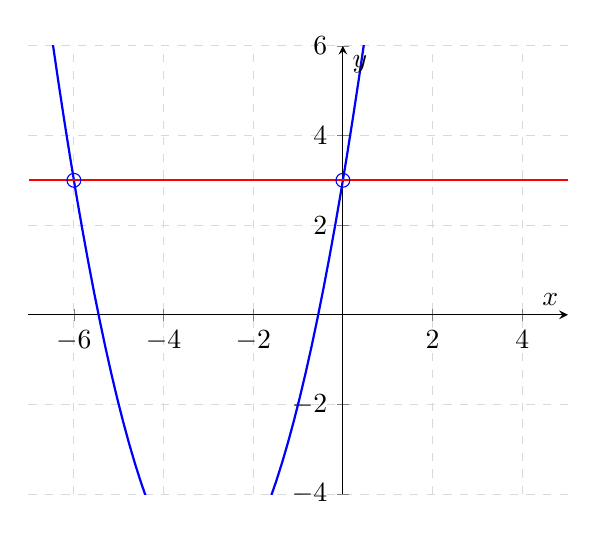
\begin{tikzpicture}
	\begin{axis}[
	    axis lines = center,
	    xlabel = $x$,
	    ylabel = $y$,
	    xmin = -6, xmax = 4,
	    ymin = -4, ymax = 6,
	    grid = both,
	    grid style = {dashed, gray!30},
	    axis equal
	  ]
	  \addplot [domain=-7:6, samples=100, thick, blue] {x^2+6*x+3};
	  \addplot [domain=-7:6, samples=100, thick, red] {3};
	  \draw[blue] (axis cs:0,3) circle (2.5pt);
	  \draw[blue] (axis cs:-6,3) circle (2.5pt);
	\end{axis}
      \end{tikzpicture}
    \end{center}
  \item $-2x^2 + 1 \quad g(x) = 3x + 2$ \\
    $-2x^2 + 1 = 3x + 2$ \\
    $0 = 2x^2 + 3x - 1 + 2$ \\
    $0 = 2x^2 + 3x + 1$ \\
    \begin{center}
      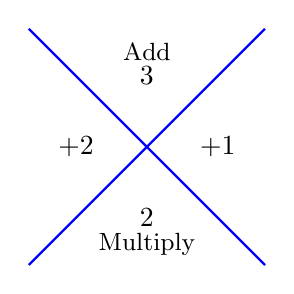
\begin{tikzpicture}[scale=1.5, auto, >=stealth]
	\draw[thick, blue] (-1, 1) -- (1, -1);
	\draw[thick, blue] (-1, -1) -- (1, 1);
	\node at (0, 0.6) {$3$};
	\node at (0, -0.6) {$2$};
	\node at (-0.6, 0) {$+2$};
	\node at (0.6, 0) {$+1$};
	\node at (0, 0.6) [above=2pt] {\small Add};
	\node at (0, -0.6) [below=2pt] {\small Multiply};
      \end{tikzpicture}
    \end{center}
    $0 = (x + 1)(2x + 1)$ \\
    $x + 1 = 0, 2x + 1 = 0$ \\
    $x = -1, x = -\frac{-1}{2}$ \\
    $$(-1, -1) (-\frac{1}{2}, \frac{1}{2})$$
    \begin{center}
      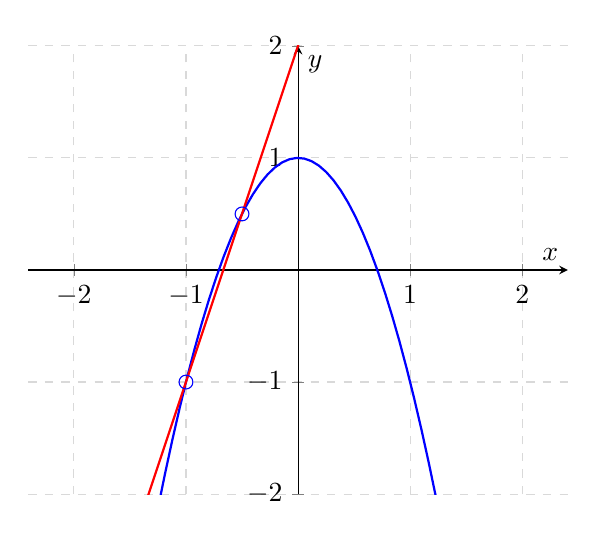
\begin{tikzpicture}
	\begin{axis}[
	    axis lines = center,
	    xlabel = $x$,
	    ylabel = $y$,
	    xmin = -2, xmax = 2,
	    ymin = -2, ymax = 2,
	    grid = both,
	    grid style = {dashed, gray!30},
	    axis equal
	  ]
	  \addplot [domain=-7:6, samples=200, thick, blue] {-2*(x^2)+1};
	  \addplot [domain=-7:6, samples=200, thick, red] {3*x+2};
	  \draw[blue] (axis cs:-1,-1) circle (2.5pt);
	  \draw[blue] (axis cs:-0.5,0.5) circle (2.5pt);
	\end{axis}
      \end{tikzpicture}
    \end{center}
  \item $f(x) = x^2 - x + 1 \quad g(x) = 2x^2 - 3x - 14$ \\
    $x^2 - x + 1 = 2x^2 - 3x - 14$ \\
    $0 = -x^2 + 2x^2 + x - 3x - 1 - 14$ \\
    $0 = x^2 - 2x - 15$ \\
    \begin{center}
      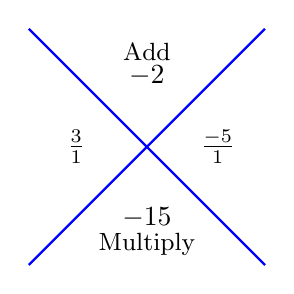
\begin{tikzpicture}[scale=1.5, auto, >=stealth]
	\draw[thick, blue] (-1, 1) -- (1, -1);
	\draw[thick, blue] (-1, -1) -- (1, 1);
	\node at (0, 0.6) {$-2$};
	\node at (0, -0.6) {$-15$};
	\node at (-0.6, 0) {$\frac{3}{1}$};
	\node at (0.6, 0) {$\frac{-5}{1}$};
	\node at (0, 0.6) [above=2pt] {\small Add};
	\node at (0, -0.6) [below=2pt] {\small Multiply};
      \end{tikzpicture}
    \end{center}
    $0 = (x + 3)(x - 5)$ \\
    $x + 3 = 0, x - 5 = 0$ \\
    $x = -3, x = 5$ \\
    $$(-3, 13) (5, 21)$$
    \begin{center}
      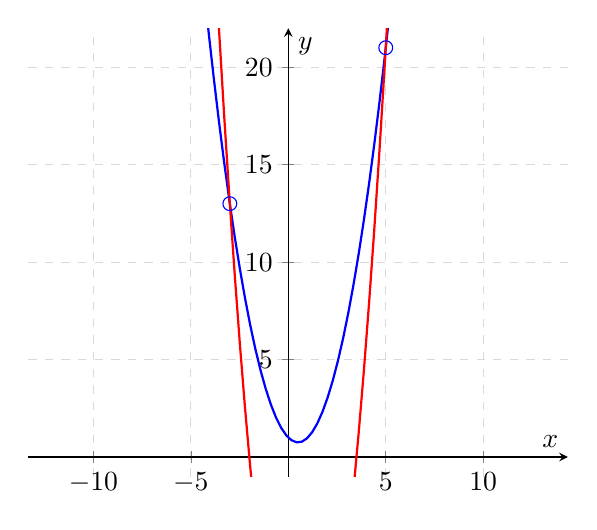
\begin{tikzpicture}
	\begin{axis}[
	    axis lines = center,
	    xlabel = $x$,
	    ylabel = $y$,
	    xmin = -4, xmax = 5,
	    ymin = -1, ymax = 22,
	    grid = both,
	    grid style = {dashed, gray!30},
	    axis equal
	  ]
	  \addplot [domain=-7:6, samples=50, thick, blue] {x^2-x+1};
	  \addplot [domain=-7:6, samples=50, thick, red] {2*x^2-3*x-14};
	  \draw[blue] (axis cs:-3,13) circle (2.5pt);
	  \draw[blue] (axis cs:5,21) circle (2.5pt);
	\end{axis}
      \end{tikzpicture}
    \end{center}
  \end{enumerate}
\end{example}
